\documentclass[10pt]{article}
\usepackage[T1]{fontenc}
\usepackage{array}

\newcolumntype{L}[1]{>{\raggedright\let\newline\\\arraybackslash\hspace{0pt}}m{#1}}
\newcolumntype{C}[1]{>{\centering\let\newline\\\arraybackslash\hspace{0pt}}m{#1}}
\newcolumntype{R}[1]{>{\raggedleft\let\newline\\\arraybackslash\hspace{0pt}}m{#1}}
\usepackage{lmodern}
\usepackage{tikz}
\usetikzlibrary{shapes.geometric, arrows}
\usetikzlibrary{positioning}
\usepackage[most]{tcolorbox}
\usepackage{hyperref}
\usepackage{geometry} 
\usepackage{xpatch}
\usepackage{xcolor}
\usepackage{listings}
\usepackage{realboxes}
\usepackage{subfig}
\usepackage{float}
\geometry{a4paper, left=10mm, right=10mm, top=20mm} 

% Set TikZ styles
\tikzstyle{arrow} = [thick,->,>=stealth]
\tikzstyle{doublearrow} = [thick,<->,>=stealth]
\tikzstyle{startstop} = [rectangle, rounded corners, minimum width=3cm, minimum height=1cm,text centered, draw=black, fill=red!30]
\tikzstyle{io} = [trapezium, trapezium left angle=70, trapezium right angle=110, minimum width=3cm, minimum height=1cm, text centered, draw=black, fill=blue!30]
\tikzstyle{process} = [rectangle, minimum width=3cm, minimum height=1cm, text centered, draw=black, fill=orange!30]
\tikzstyle{decision} = [diamond, minimum width=3cm, minimum height=1cm, text centered]

% Do not indent first line of new paragraphs not following sections
\setlength\parindent{0pt}

% \usepackage{amsmath} % \usepackage is a command that allows you to add functionality to your LaTeX code
\usepackage{titling}
\usepackage{graphicx} % the demo option is just for the example

\graphicspath{ {.././images/} } % Where to find images

% Set inline code style
\definecolor{code_background_color}{rgb}{0.8,0.8,0.8}
\lstset{
  basicstyle=\ttfamily,
  backgroundcolor=\color{code_background_color},
  columns=fullflexible,
  breaklines=true,
  postbreak=\mbox{\textcolor{red}{$\hookrightarrow$}\space},
}

\makeatletter
\xpretocmd\lstinline{\Colorbox{code_background_color}\bgroup\appto\lst@DeInit{\egroup}}{}{}
\makeatother

% Setup document link styles
\hypersetup{
    colorlinks,
    citecolor=black,
    filecolor=black,
    linkcolor=blue,
    urlcolor=blue
}

%textmarker style from colorbox doc
\tcbset{textmarker/.style={%
        enhanced,
        parbox=false,boxrule=0mm,boxsep=0mm,arc=0mm,
        outer arc=0mm,left=6mm,right=3mm,top=7pt,bottom=7pt,
        toptitle=1mm,bottomtitle=1mm,oversize}}


% define new colorboxes
\newtcolorbox{hintBox}{textmarker,
    borderline west={6pt}{0pt}{yellow},
    colback=yellow!10!white}
\newtcolorbox{importantBox}{textmarker,
    borderline west={6pt}{0pt}{red},
    colback=red!10!white}
\newtcolorbox{noteBox}{textmarker,
    borderline west={6pt}{0pt}{green},
    colback=green!10!white}
\newtcolorbox{infoBox}{textmarker,
    borderline west={6pt}{0pt}{blue},
    colback=blue!10!white}
  

% define commands for easy access
\newcommand{\info}[1]{\begin{infoBox} \textbf{Info:} #1 \end{infoBox}}
\newcommand{\note}[1]{\begin{noteBox} \textbf{Note:} #1 \end{noteBox}}
\newcommand{\warning}[1]{\begin{hintBox} \textbf{Warning:} #1 \end{hintBox}}
\newcommand{\important}[1]{\begin{importantBox} \textbf{Important:} #1 \end{importantBox}}

% Show NSPanelManager logo on first page above title
\pretitle{%
  \begin{center}
  \LARGE
  
\includegraphics{logo.png}\\[\bigskipamount]
}
\posttitle{\end{center}}

\title{User \& Technical reference manual} % Sets article title
\author{} % Sets authors name
\date{} % Sets date for date compiled

% The preamble ends with the command \begin{document}
\begin{document} % All begin commands must be paired with an end command somewhere
    \maketitle % creates title using information in preamble (title, author, date)

    \clearpage
    \tableofcontents
    \clearpage
    \section{Introduction} % creates a section
    NSPanel Manager is a custom software solution for the Sonoff NSPanel (not the NSPanel pro). The software is designed to be easy to use on a day to day basis and to easily manage multiple NSPanels around your home.
    The interface on the NSPanel itself has been designed to be intuitive to use for people of all ages and backgrounds.
    \bigbreak
    All the NSPanel that are installed with the NSPanel Manager solution communicate back to a Docker container that is used to manage the panels, NSPanel Manager specific solutions and also all communication back and forth to/from Home Assisant and/or OpenHAB.
    \bigbreak
    \info{For the latest release of this document, please check the GitHub page \href{https://github.com/NSPManager/NSPanelManager}{here}.}

    \clearpage
    \section{Quick start guide}
    \subsection{Container installation/update}
    \subsubsection{Windows}
    \important{There are currently problems running NSPanel Manager container on WSL2 as WSL2 does not handle networking properly. For more information, see the following \href{https://github.com/microsoft/WSL/issues/4150}{issue} on GitHub.}
    If you wish to run the NSPanel Manager container on Windows the current solution is to run it in a virtual machine. When you have your virtual machine up and running, you can follow the "Standalone docker container" installation below.
    \subsubsection{Standalone Docker container}
    \label{sec:standalone_docker_container}
    \textbf{Installation}\newline
    Prerequisites:
    \begin{itemize}
      \item Working Docker installation.
    \end{itemize}
    The pre-built container image is available on Docker hub as several different architectures, the following architectures are available:
    \begin{itemize}
      \item armhf
      \item armv7
      \item aarch64
      \item i386
      \item amd64
    \end{itemize}
    In order to run one of these images, issue the docker run command with the appropriate image for your hardware. The following is an example on how to start the image on a x64 PC with timezone Europe/Stockholm and store the data from the container in the "/nspmdata/"-directory:
    \begin{lstlisting}[language=bash]
    docker run --name nspanelmanager -e TZ=Europe/Stockholm -v \
    "/nspmdata/":"/data/" \
    -d -p 8000:8000 nspanelmanager/nspanelmanager-amd64:latest
    \end{lstlisting}
    \important{All the data for the container will be stored in the directory mapped to /data/ in the container, in the example above this is the /nspmdata/-directory on your machine.}
    If you wish to manually build and run the container or change options or settings, see below for \hyperref[sec:advanced_setup]{advanced setup}.
    \bigbreak
    \textbf{Update an existing installation}\newline
    When a new updated is released, do the following to update the standalone docker container:
    \important{Create a backup of the "nspanelmanager\_db.sqlite3"-file in the /nspmdata/-directory as it contains all settings and stored data for the container.}
    In order to update to the latest version of the container you have to remove the current image and recreate it. Perform the following in order to update:
    \begin{itemize}
      \item Run \lstinline[language=bash]{docker rm -f nspanelmanager}.
      \item Run \lstinline[language=bash]{docker rmi nspanelmanager}.
      \item Redo the installation steps \hyperref[sec:standalone_docker_container]{above} and make sure to point to the same data\_dir as previously.
    \end{itemize}
    \info{Container management can be made much easier with the help of tools like \href{https://www.portainer.io/}{portainer}.}

    \subsubsection{Home Assistant add-on}
    \textbf{Installation}
    \begin{itemize}
      \item In the Home Assistant web interface, navigate to Settings $\rightarrow$ Add-ons $\rightarrow$ Add-on store.
      \item In the upper right corner, press the three dots and choose "Repositories".
      \item Add \textbf{https://github.com/NSPManager/NSPanelManager} to the list of repositories and close the dialog.
      \item Select the "NSPanel Manager" add-on and install it.
      \item Check that the add-on should start automatically.
      \item Start the add-on.
    \end{itemize}
    \bigbreak
    \textbf{Update an existing installation}\newline
    When a new update is release, do the following to update the container currently installed in Home Assistant:
    \begin{itemize}
      \item In the Home Assistant web interface, navigate to Settings $\rightarrow$ Add-ons and check for updates.
      \item Select the "NSPanel Manager"-add-on and choose to update it.
    \end{itemize}


    \subsection{Container settings}
    \begin{figure}[H]
    \centering
    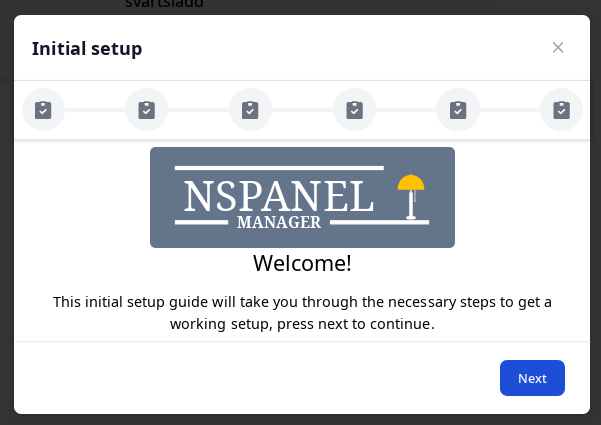
\includegraphics[height=5cm,keepaspectratio]{initial_setup_popup.png}
    \caption{Initial setup}%
    \end{figure}
    When first logging in to the NSPanel Manager web interface you will be greeted by a \textbf{Initial setup} dialog. This guide will help you setup the required items in order to have a functional setup.
    The following is a walkthrough of what to enter:

    \begin{itemize}
      \item \textbf{Manager config}
        \begin{itemize}
          \item \textbf{Manager address} - This address is sent to NSPanel over MQTT when the request to connect with a manager. This can be loaded from the URL using the "Load from URL" button. This address needs to be reachable by all NSPanels.
          \item \textbf{Manager port} - This port that will be used to connect to the address above.
        \end{itemize}
      \item \textbf{MQTT config}
        \begin{itemize}
          \item \textbf{MQTT address} - The address to your MQTT broker. If you are running your MQTT broker as an addon to Home Assistant, enter you Home Assistant address (only IP).
          \item \textbf{MQTT port} - The port to connect to your MQTT broker.
          \item \textbf{MQTT username} - The username to authenticate to your MQTT broker. Leave empty if you don\'t use authentication.
          \item \textbf{MQTT password} - The password to authenticate to your MQTT broker. Leave empty if you don\'t use authentication.
        \end{itemize}
      \item \textbf{Home Assistant config (optional)}
        \begin{itemize}
          \item \textbf{Home Assistant address} - The address to your Home Assistant instance. This address should include "http" or "https" in the beginning and ":8123" (change to your port) at the end.
          \item \textbf{Home Assistant token} - The long lived access token used to authenticate to Home Assistant.
        \end{itemize}
      \item \textbf{OpenHAB (optional)}
        \begin{itemize}
          \item \textbf{OpenHAB address} - The address to your OpenHAB instance. This address should include "http" or "https" in the beginning and ":8123" (change to your port) at the end.
          \item \textbf{OpenHAB token} - The access token used to authenticate to OpenHAB.
        \end{itemize}
    \end{itemize}

    Once the above is completed, continue on with \hyperref[sec:nspanel_flashing]{NSPanel flashing} to flash the NSPanel Manager firmware on to a NSPanel.

    \subsection{NSPanel flashing}
    \label{sec:nspanel_flashing}
    Prerequisites:
    \begin{itemize}
      \item Working TTL flasher for 3.3V.
      \item Working serial setup for your PC and known serial port (in Windows known as COM-port).
    \end{itemize}
    In order to connect to the NSPanel and be able to flash it, you must dismantle it. For a guide on how to dismantle and connect your serial flasher to the NSPAnel, refer to \href{https://www.youtube.com/watch?v=p-AK4o5jOSI}{this} guide from MarkWattTech.
    \subsubsection{Flashing with Espressif ESP32 DOWNLOADER TOOL (Windows only)}
    To flash the panel, perform the following:
    \begin{itemize}
      \item Download the tool from Espressif from \href{https://www.espressif.com/en/support/download/other-tools}{here}.
      \item Open the tool and choose to flash an ESP32 chip.
      \item Check one checkbox and select the "merged\_flash.bin"-file in the "docker/web/nspanelmanager/"-directory.
      \item Enter "0x0" as the upload address.
      \item Connect your flasher to the NSPanel and press "START".
    \end{itemize}
    \begin{center}
    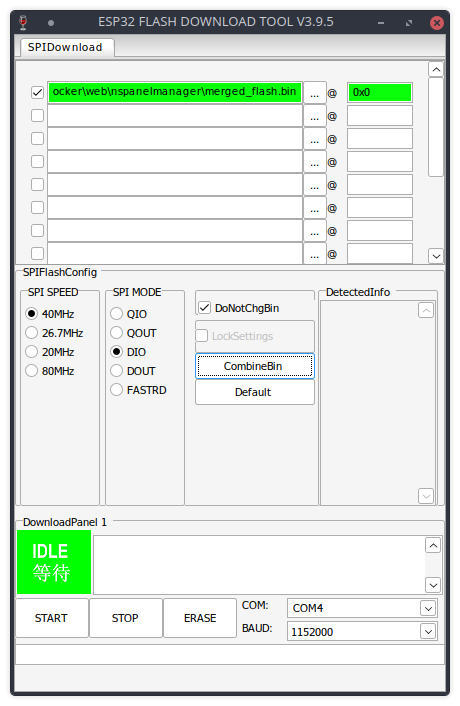
\includegraphics[scale=0.4]{esp_flash_download_tool.png}
    \end{center}
    \subsubsection{Flashing with ESPtool (all operating systems)}
    By installing esptool it is possible to upload the merged flash using the command line. Do the following:
    \begin{itemize}
      \item Open a terminal.
      \item Navigate to the "docker/web/nspanelmanager/"-directory.
      \item To determine if you have selected the right port, run \lstinline[language=bash]|esptool.py flash_id --port <port>|. You will have to replace "<port>" with the actual port connected to the NSPanel. This will do a check and see if the tool can communicate with the NSPanel.
      \item Run \lstinline[language=bash]|esptool.py --baud 921600 --port /dev/ttyUSB0 write_flash 0x0 merged_flash.bin|. You will have to replace "/dev/ttyUSB0" with the actual port connected to the NSPanel.
      \info{On Windows it might be just "esptool" without the ".py" at the end.}
      \info{On Windows "/dev/ttyUSB0" will have to be replaced by something like "COM4". If using MacOS or Linux the port will be something similar to "/dev/ttyUSB0".}
    \end{itemize}
    After the flashing is complete you can continue with \hyperref[sec:nspanel_configuration]{NSPanel configuration}.
 
    \subsection{NSPanel configuration}
    \label{sec:nspanel_configuration}
    To configure the NSPanel, do the following:
    \begin{itemize}
      \item Power up the panel.
      \warning{If you have flashed multiple NSPanels, power them up one at a time as they will all have the same WiFi access point name.}
      \info{The GUI file has not been flashed yet so there will not be any visible change on the NSPanel screen.}
      \item Connect to the new WiFi network "NSPMPanel" when the panel has started. It's an open WiFi network ie. no password.
      \item When connected to the new WiFi network, make sure your device does not disconnect because it doesn't detect internet access. Then open a browser and navigate to "http://192.168.1.1".
      \info{There have been issues when using Android and the Chrome browser that it sometimes just shows a blank page. If this is the case, either use a different browser (E.g. Firefox) or another device with WiFi to access the web page.}
      \item Enter a friendly name for the NSPanel.
      \note{This name is only used to register the NSPanel the first time. After the panel has been registered the name has to be changed from the manager web interface.}
      \item Enter WiFi name and password.
      \item Enter MQTT address and port. If you are using authentication for MQTT, enter username and password as well.
      \note{If you are running the MQTT server as an add-on to Home Assistant, enter the IP-address of your Home Assistant server.}
      \item Press the "Save" button on the bottom of the page. The panel will reboot and try to connect to the WiFi network.
      \info{If the panel fails to connect to the WiFi network for three minutes it will revert back and start the access point again. It will periodically scan for the configured WiFi and, if it detects that the configured WiFi has come back, it will reboot and connect to it.}
      \item Connect to your WiFi again and go to the NSPanel Manager web interface. If all things are working and setup correctly the panel should show up in the list of panels on the first page. You will then have to accept or deny the panel access into the manager.
      \info{If this is a US NSPanel version then it has to be set in the panel settings. Press the name of the NSPanel in the list and check the "Is US panel"-checkbox.}
      \item Flash the new GUI file to the panel by pressing the "Actions"-button on the right and select "Update GUI".
      \note{The flashing of the GUI file may be finicky and might require multiple tries before it succeeds. If it fails and reboots or you see a "System data error", just try again.}
    \item Continue on to create new rooms and add entities to your configuration. Continue with the section on the web interface and how it work \hyperref[sec:nspanelmanager_web_interface]{here}.
    \end{itemize}

    \clearpage
    \section{NSPanel Manager web interface}
    \label{sec:nspanelmanager_web_interface}
    This chapter describes all pages available in the web interface and all settings that can be made. The web interface also links to specific sections in this chapter for help information.
    \subsection{First page}

    \begin{figure}[H]
    \centering
    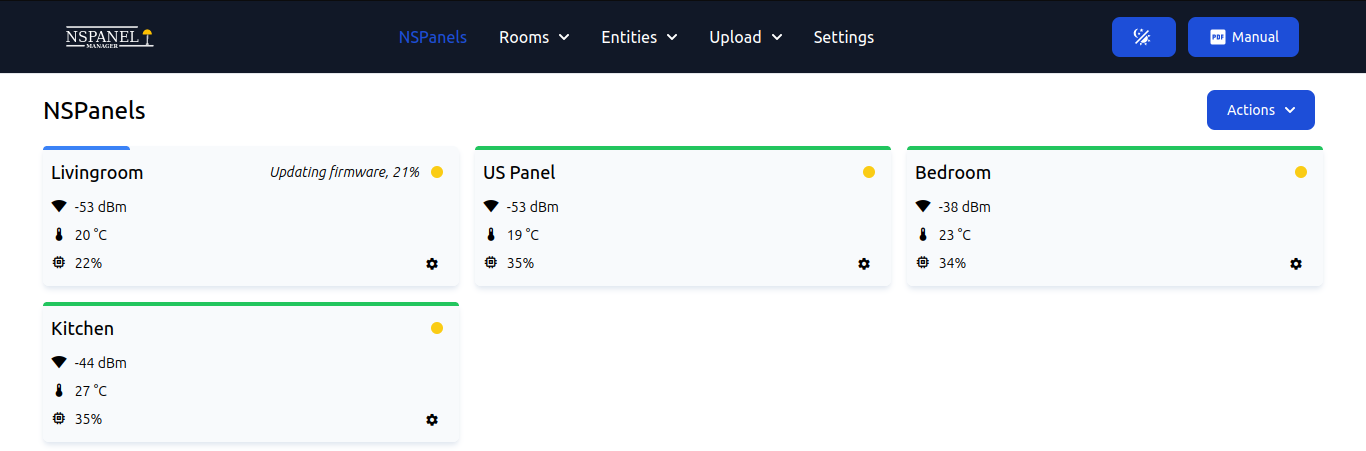
\includegraphics[width=\textwidth,height=\textheight,keepaspectratio]{index_page.png}
    \caption{First page}%
    \end{figure}

    The first page is used to get an overview of each registered NSPanel as well as perform actions on each panel individually or all at once. These actions are available in the menu accessed by pressing the cog. The available actions are:
    \begin{itemize}
      \item \textbf{Reboot} - Reboot the NSPanel.
      \item \textbf{Settings} - Navigate to the \hyperref[sec:nspanel_page]{NSPanel settings page} where individual settings for the panel can be made. This page can also be accessed by pressing the name of the panel.
      \item \textbf{Visit} - Visit the web page that is on the panel itself. This is the same page that was used to enter initial WiFi and MQTT information.
      \item \textbf{Firmware update} - Send a command to the NSPanel to update the firmware. The firmware will be downloaded from the manager.
      \item \textbf{GUI update} - Send a command to the NSPanel to update the screen. The screen firmware will be downloaded from the manager.
      \item \textbf{Delete} - Delete the nspanel from the manager.
    \end{itemize}

    There is also the "Actions"-button on the top right where you can perform some of the actions from the list above to all panels which are online. There is also an option to \textbf{Restart MQTTManager} which will restart the 
    core component that handles all communication between different components of the NSPanel Manager software.

    \hypertarget{sec:nspanel_page}{}
    \subsection{NSPanel page}
    \label{sec:nspanel_page}
    \begin{figure}[H]
    \centering
    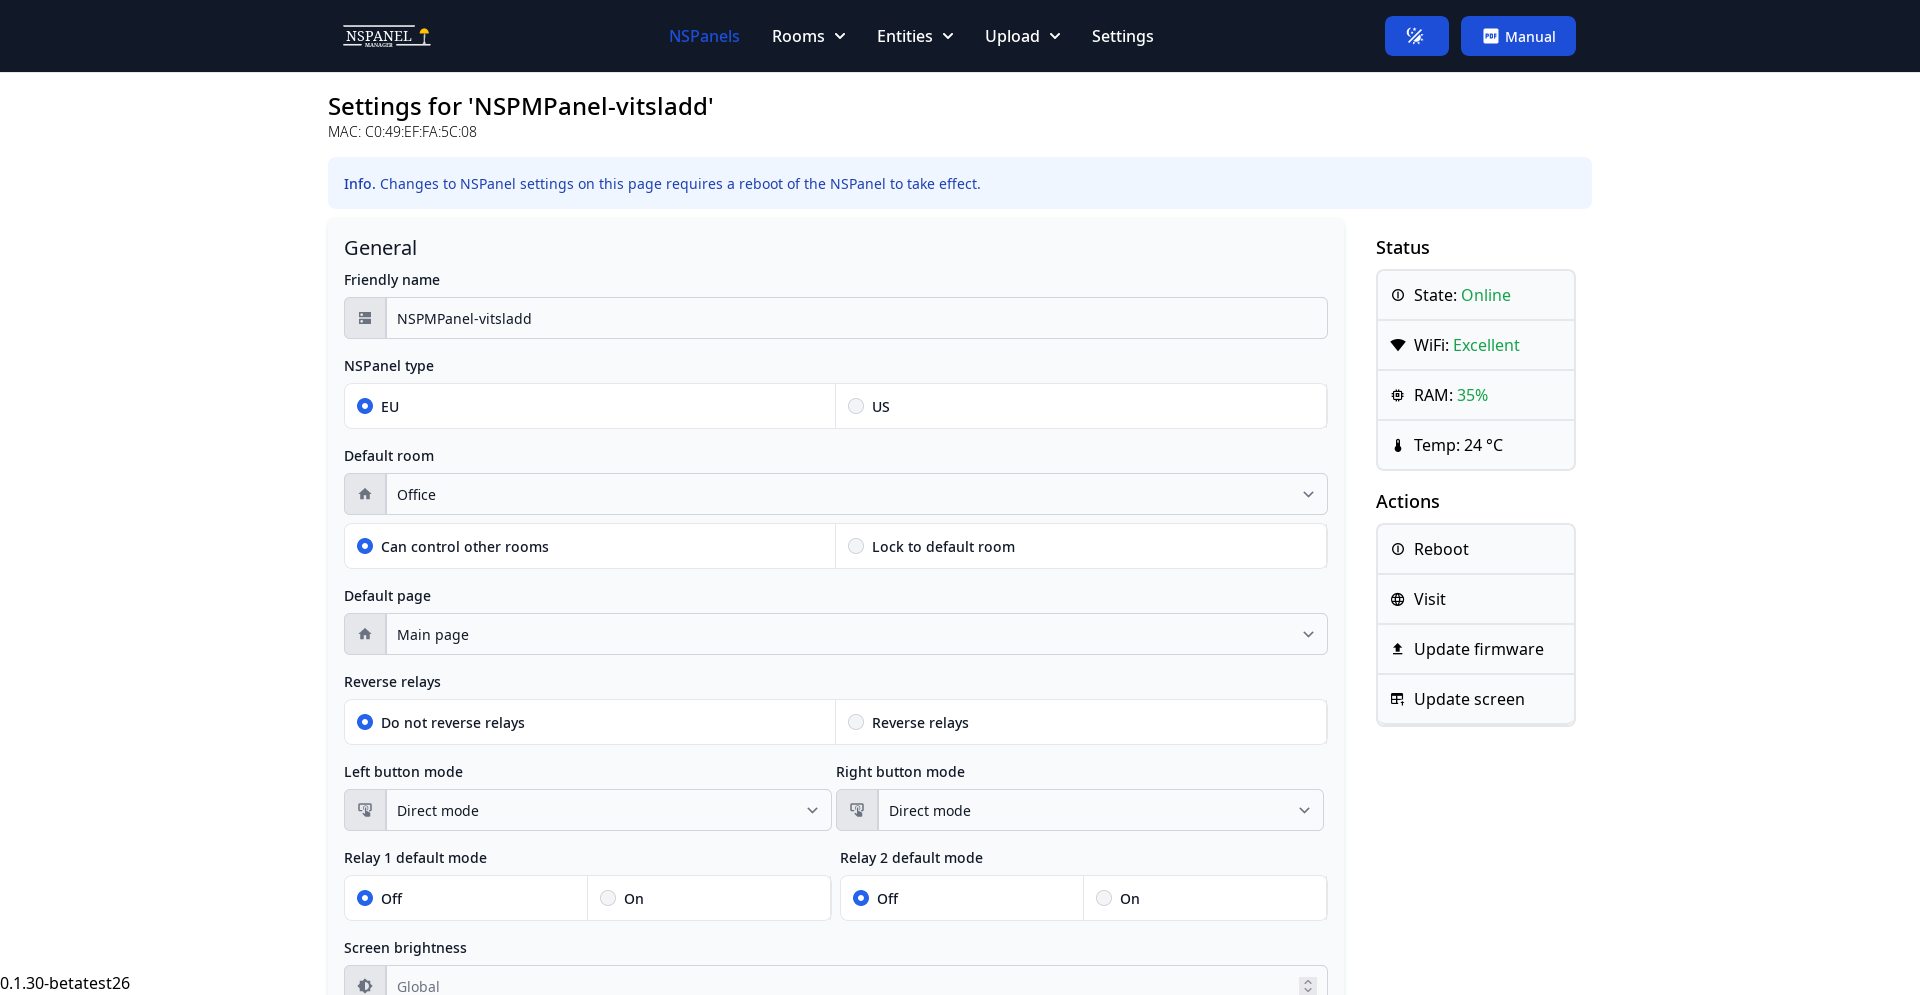
\includegraphics[scale=0.25,keepaspectratio]{nspanel_page.png}
    \caption{NSPanel page}%
    \end{figure}

    The NSPanel settings page is used to configure specific settings for each individual NSPanel. This includes things like NSPanel type (EU/US), the room it is installed in, name and so on. See below for a complete list of options.
    The page can also be used to look at the live stream of logs from the NSPanel and send commands to the panel. What is displayed in the log view is dependent on what log level is configured on the settings page on the panel itself.
    \subsubsection{Available options}
    Available options for each individual NSPanel are:

    \begin{itemize}
      \item \textbf{Friendly name} - The name of the NSPanel.
      \item \textbf{NSPanel type} - The type of NSPanel, either \textbf{EU} or \textbf{US}.
      \item \textbf{Default room} - Select the default room for the NSPanel. This is the room that will be selected in the GUI after the NSPanel has booted and after the screensaver has been active. It is also possible to lock the NSPanel to the default room so that it can't control entities in other rooms.
      \item \textbf{Default page} - Select a different default page. Available options are:
      \begin{itemize}
        \item \textbf{Main page} - The default page with sliders and buttons for light control.
        \item \textbf{Scenes page} - The page where scenes can be activated and saved.
        \item \textbf{Room page} - The page that is used to control individual entities.
      \end{itemize}
      \item \textbf{Reverse relays} - Reverse the relays. This is the same as switching places of the cables on the back of the NSPanel. All actions meant for relay 1 will be applied to relay 2 and vice versa.
      \item \textbf{Left/Right Button mode} - Change the mode of a button. Available options are:
      \begin{itemize}
        \item \textbf{Direct mode} - The buttons controls the relay directly. No WiFi is needed.
        \item \textbf{Detached mode} - Detached mode controls a button via you selected home automation platform. This also exposes the option "Left/Right button controls light" where you select which entity it controls.
        \item \textbf{Custom MQTT} - This mode can be used to send a custom message on a custom MQTT topic.
        \item \textbf{Follow mode} - When the button is pressed the relay is engaged, when the button is release the relay is disconnected.
      \end{itemize}
      \item \textbf{Relay 1/2 default mode} - Select the default mode of the relay when the NSPanel starts.
      \item \textbf{Register relay 1/2 as}:
        \begin{itemize}
          \item \textbf{Switch} - The relay will be registered to Home Assistant as a switch entity.
          \item \textbf{Light} - The relay will be registered to Home Assistant as a light entity.
        \end{itemize}
      \item \textbf{Screen brightness} - The brightness of the screen when on (1-100\%).
      \item \textbf{Screensaver brightness} - The brightness of the screen when the screensaver is active (0-100\%). A value of 0 means that the screen is off.
      \item \textbf{Screensaver mode} - Select what to display on the screensaver. Available options are:
      \begin{itemize}
        \item \textbf{Global (use global setting)} - Use whatever is set in the "settings" section of the NSPanel Manager.
        \item \textbf{Show with background (clock, date and weather)} - Show the screensaver with background image with current and forecast weather, time and date.
        \item \textbf{Show without background (clock, date and weather)} - Show the screensaver with a black background with current and forecast weather, time and date.
        \item \textbf{Show with background (no weather)} - Show the screensaver with background image but only time and date.
        \item \textbf{Show without background (no weather)} - Show the screensaver with a black background but only time and date.
        \item \textbf{No screensaver (turn off screen)} - Make the screen completely black when not in use.
      \end{itemize}
      \item \textbf{Temperature calibration} - Calibrate the internal temperature sensor. Enter a negative value to bring the reported temperature down and vice versa.
    \end{itemize}
    
    \hypertarget{sec:room_page}{}
    \subsection{Room page}
    \label{sec:room_page}
    This section will describe how to manage rooms. Most of the configuration done with NSPanel Manager will be done in rooms, please read this chapter for a full understanding on how to work with rooms.

    \begin{figure}[H]
    \centering
    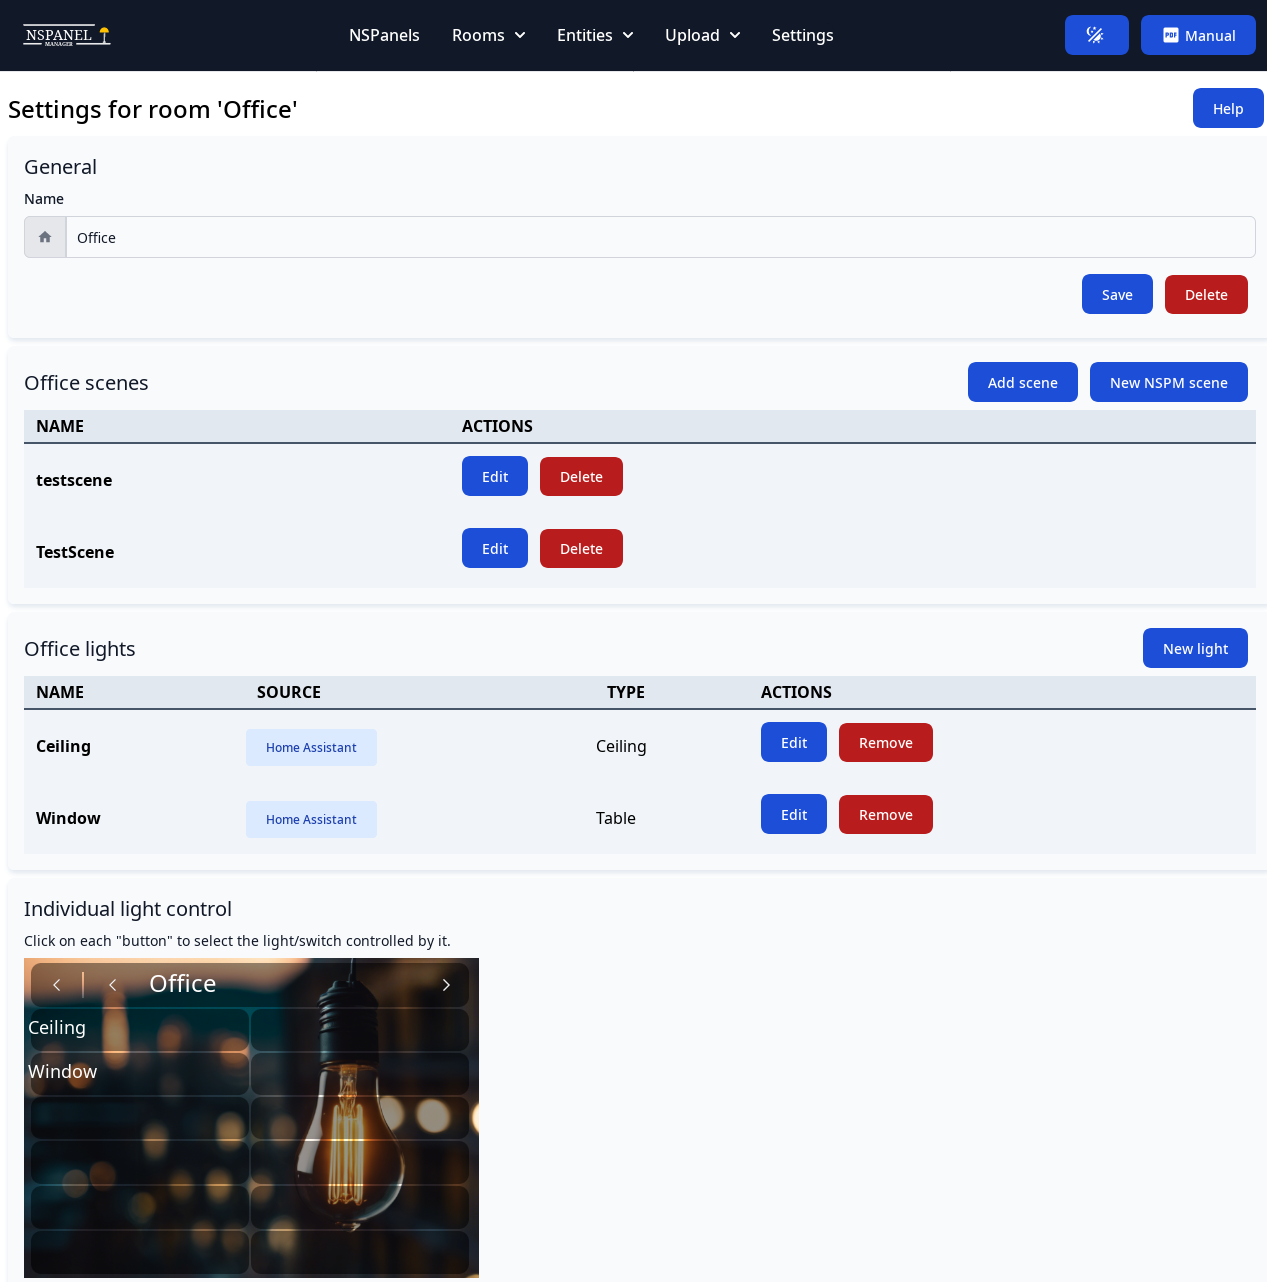
\includegraphics[width=\textwidth,height=\textheight,keepaspectratio]{room_page.png}
    \caption{Room page}%
    \end{figure}
    \subsubsection{Scenes}
    You can choose to use scenes from Home Assistant or OpenHAB though these scenes will not be able to be saved on the fly. This is something that the NSPanel Manager scenes can perform internally.
    
    The NSPanel Manager scenes are easy enough to use. Simply create a scene in the room page and they will be available in the "Scenes"-list for the room on all NSPanels.
    \\ To save a scene, on the NSPanel hold the save button for the scenes for 3 seconds to save all the states of lights \textbf{currently added to the room}.
    \\ To recall/activate a scene, on the NSPanel press the name of the scene and all the saved light states will be restored for that scene.
    \note{If a light was added after a scene was saved, that light is not affected by that scenes until the scene is saved again.}

    \subsubsection{Lights}
    To add a new light, simply press the "Add new light"-button. When doing so, a list of all lights and switches gathered from Home Assistant and OpenHAB will be shown. Simply search or scroll to find the desired light and press it.
    \begin{figure}[H]
    \centering
    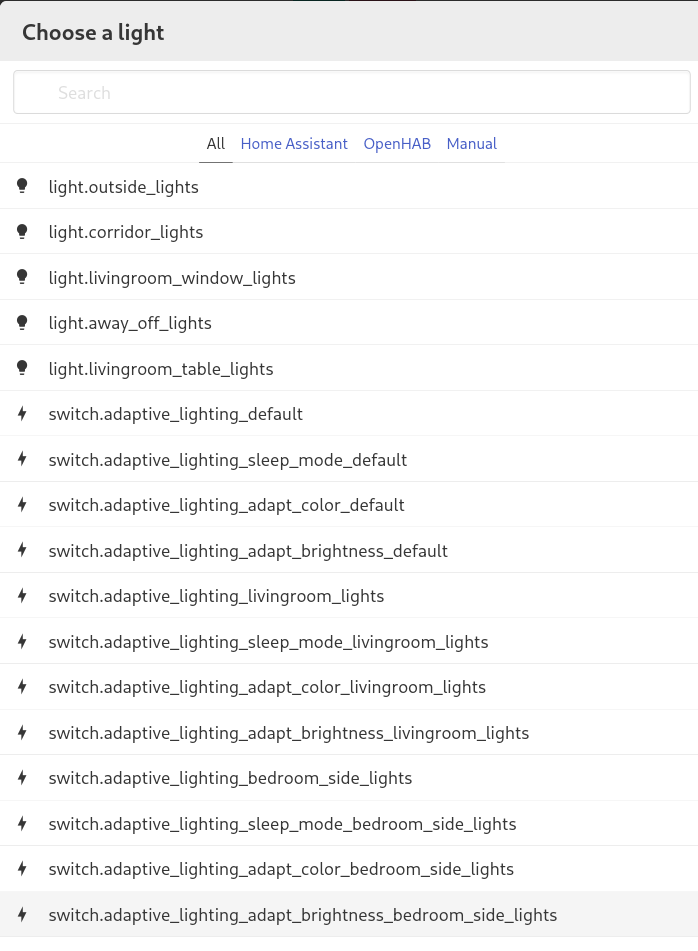
\includegraphics[scale=0.25]{add_new_light.png}
    \caption{Adding a new light to a room}%
    \end{figure}
    
    When done, a new screen will show up and depending on if the selected entity was from Home Assistant or OpenHAB difference options will be shown.
    \begin{figure}[H]
    \centering
    \subfloat[\centering Home Assistant]{{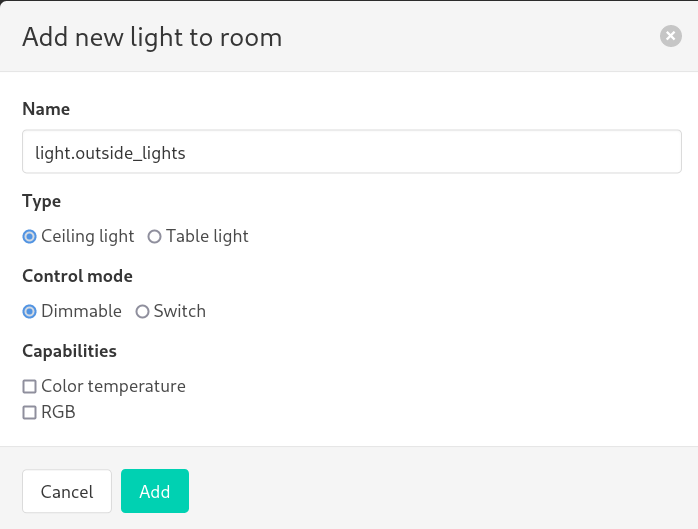
\includegraphics[width=5cm]{edit_new_light_ha.png} }}%
    \qquad
    \subfloat[\centering OpenHAB]{{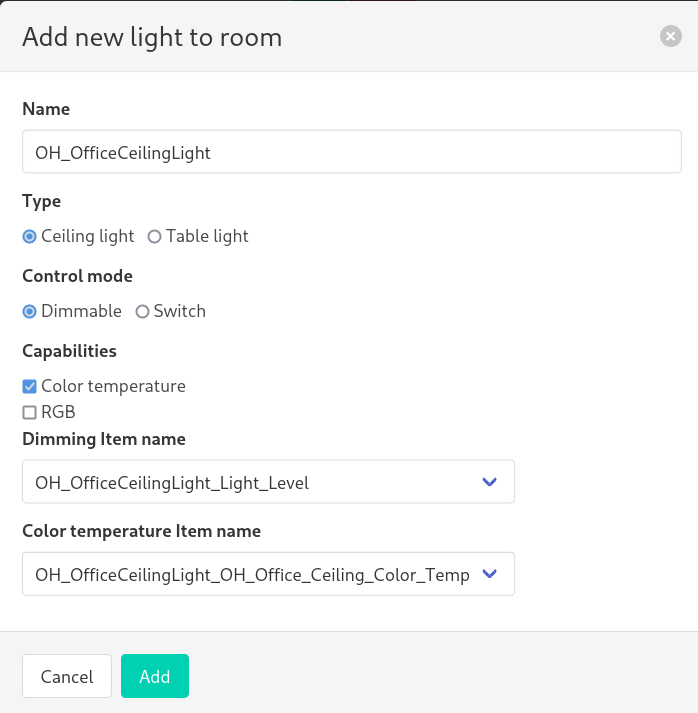
\includegraphics[width=5cm]{edit_new_light_openhab.png} }}%
    \caption{Add/Edit light}%
    \end{figure}
    
    When adding a Home Assistant entity, simply set a friendly name for it, select the type (Ceiling or Table light), select if it's a switch or dimmable light and what other capabilities it has.\\
    If you are adding an OpenHAB light or switch, things aren't as simple unfortunately. There is really no way around this and as such the user has to chose all the same settings as for Home Assistant but also has to select the appropriate OpenHAB items that corresponds to each capability of the light.

    \subsubsection{Individual light control}
    There is place for up to 12 lights (per room) to be controlled individually from the NSPanel. The image on the bottom shows a preview on how this might look. When a new light is added to the room it will automatically be assigned to the next free slot on the page. By pressing a slot with an assigned entity you can chose to assign a new entity (if any entity is unasigned) or "clear" the slot which will remove the light from the page but it will still be attached to the room.
    \info{Each entity may only be assigned to one slot. If the list of entities is empty then all entities has been assigned a slot.}


    \hypertarget{sec:relay_groups}{}
    \subsection{Relay groups}
    Relay groups are used to bind multiple NSPanels and relays together so that when one relay in the group changes state, all the relays in the group transission to the new state.


    \hypertarget{sec:weather_and_time}{}
    \subsection{Weather and Time}
    \begin{figure}[H]
    \centering
    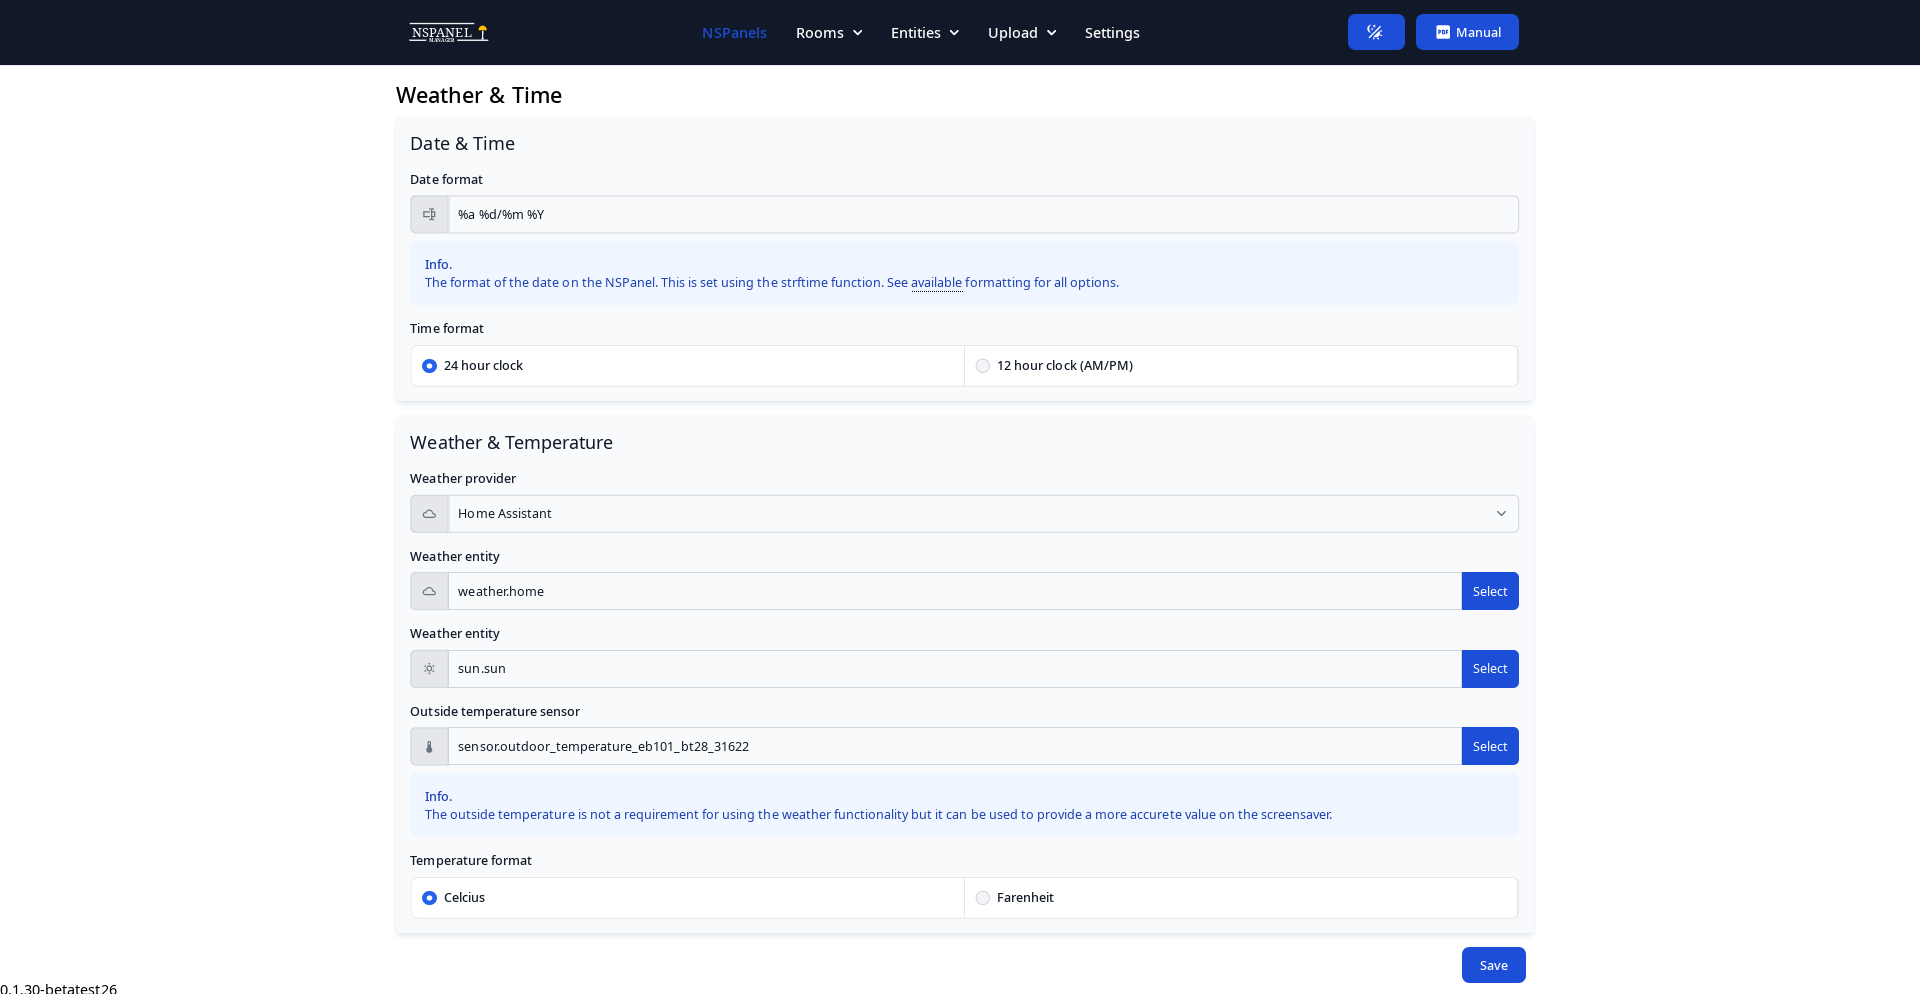
\includegraphics[scale=0.25]{weather_and_time.png}
    \caption{Weather and Time settings}%
    \end{figure}
    On the Weather \& Time page settings related to time, date and weather can be changed. Date format is configured according to the strftime function and a link to available formatting options is availabel in the information box.
    \\It is also possible to select between 24 and 12-hour clock format.

    
    To configure weather, simply press the "Search" button attached to either the "Latitude" or "Longitude" input fields and search for your city. If it does not show, you can enter your location manually.
    You can also change between celsius and fahrenheit, difference wind speed units and also difference precipitation units. You can also set the update interval for how often to pull down the current weather and the forecast from Open Meteo.
    \\
    If you wish to show temperature from a local temperature sensor available in OpenHAB, this can be selected in the \textbf{Outside temperature sensor} but it is not required.
    
    \hypertarget{sec:global_settings}{}
    \subsection{Global settings}
    These settings will apply to all NSPanels (if they do not have specific configurations), and the NSPanel Manager container. There are two things that need to be set in order to get up and running. Those are:
    \begin{enumerate}
      \item Connection details to the same MQTT server that were set in the NSPanel configuration.
      \item Connection details to Home Assistant and/or OpenHAB.
    \end{enumerate}
    \important{Failing to meet both requirements listed above will result in a non-working setup!}
    \info{If running the NSPanel Manager container as a Home Assistant add-on then the Home Assistant connection details will already be configured.}
    There are also other settings that might be worth taking a look at while here, such as global scenes that apply to all entities, showing a clock on the screensaver, how bright the NSPanels should be, the Min \& Max of color temperature and so on. Go ahead and explore by yourself.
    \begin{figure}[H]
    \centering
    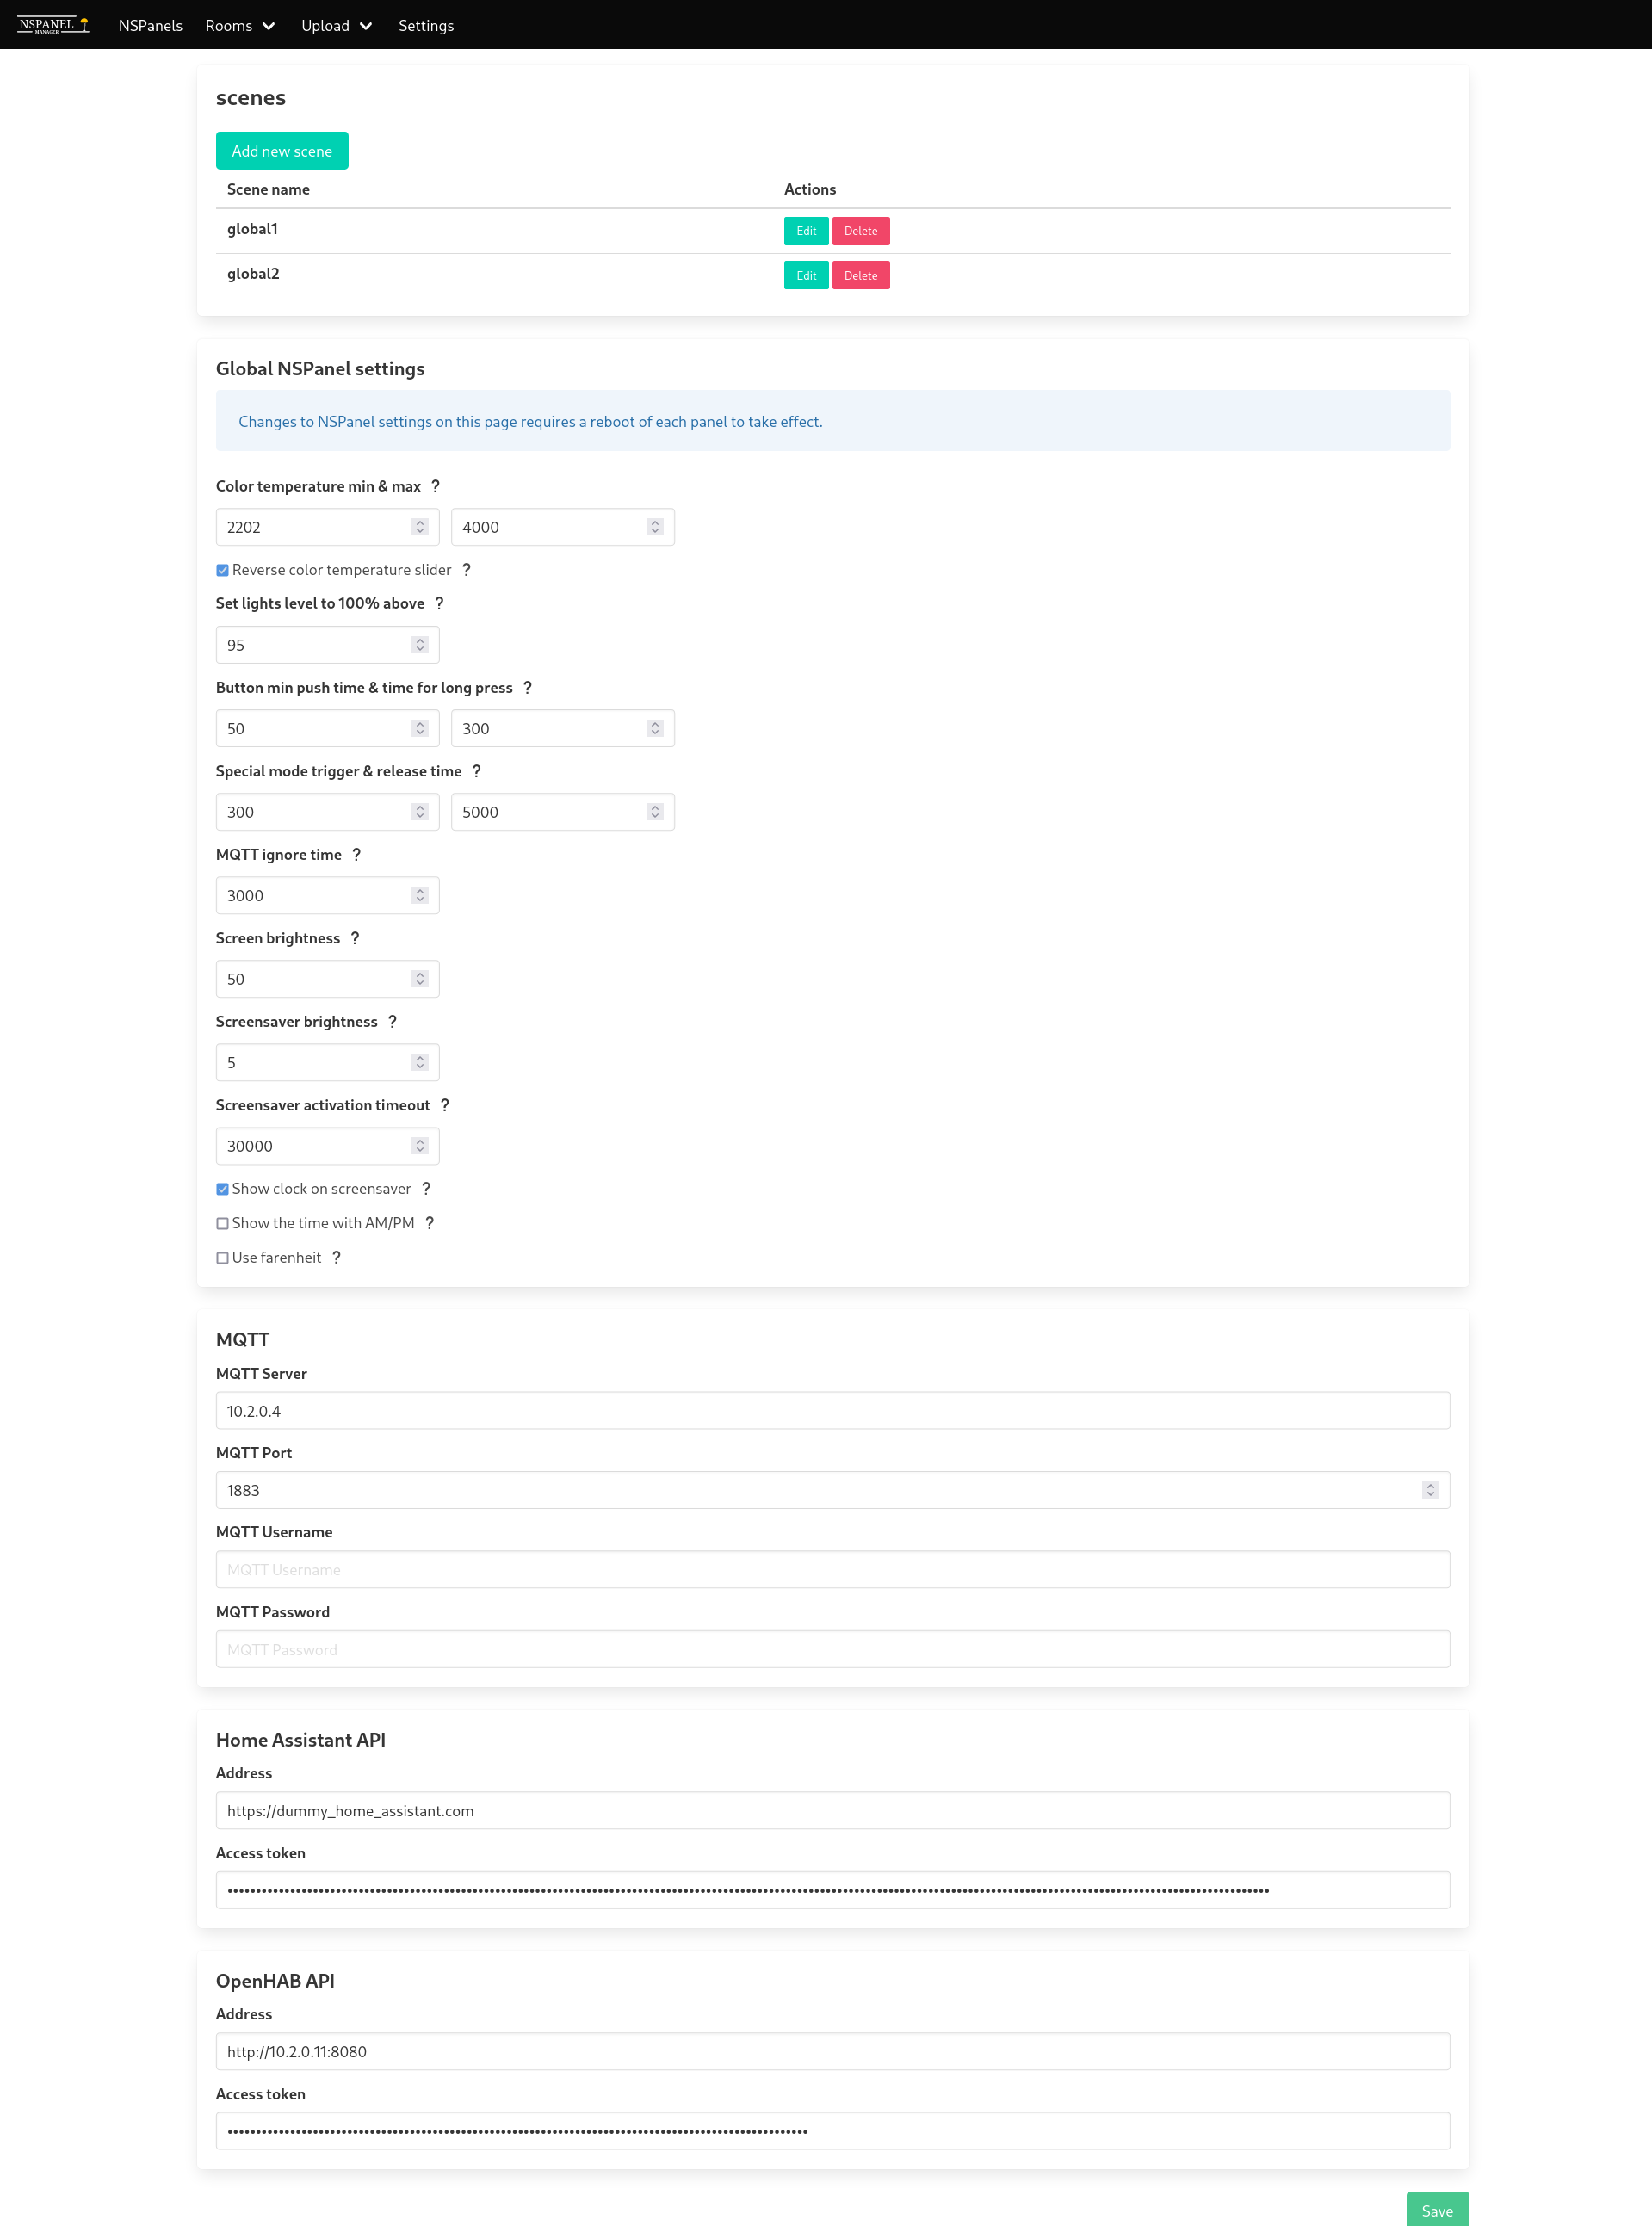
\includegraphics[scale=0.25]{settings_page.png}
    \caption{Global settings}%
    \end{figure}

    The "Global settings" section of the web interface is where you can settings that apply to all NSPanels or settings that simply are not directly related the the panels themsevles. The following options are available:
    \subsubsection{Connection settings}
    \begin{itemize}
      \item \textbf{Manager address} - The is the IP address that will be sent to each NSPanel when it boots. This address is used in the NSPanel to communicate with the manager and has to be reachable from each and every NSPanel.
      \item \textbf{Manager port} - Port to use when connecting to the above mentioned IP address.
    \end{itemize}

    \subsubsection{Logging options}
    \begin{itemize}
      \item \textbf{MQTTManager log level} - Log level for the MQTTManager background component. For more information about MQTTManager see \hyperref[sec:software_components]{Software components}. There is also a "Download"-button available in this section to download the MQTTManager log file as a .txt-file.
      \item \textbf{Number of messages to display on live log} - The number of log messages to display in the live log for each NSPanel in the NSPanel settings page.
      \item \textbf{Number of messages in buffer} - The number of log messages to keep in buffer in the MQTTManager.
    \end{itemize}

    \subsubsection{Global NSPanel settings}
    \begin{itemize}
      \item \textbf{Minimum color temperature} - The minimum kelvin to send to Home Assistant/OpenHAB.
      \item \textbf{Maximum color temperature} - The maximum kelvin to send to Home Assistant/OpenHAB.
      \item \textbf{Reverse color temperature slider} - Reverse the color temperature sliders on the NSPanel used to control color temperature on lights.
      \item \textbf{Turn on behavior} - Wether to send color temperature when turning on the light or to simply send the "turn on" command.
      \item \textbf{Raise lights to 100\% threshold} - The slider on the NSPanel can be finiky to get to reach the maximum value of 100\%. To solve this problem this option can be used to force the value to be 100\% above the given value.
      \item \textbf{Minimum button push time (ms)} - The minimum amout of time (in milliseconds) for the physical buttons to be pressed for it to register as a button press.
      \item \textbf{Minimum long press time (ms)} - The minimum amout of time (in milliseconds) for the physical buttons to be pressed for it to register as a long button press.
      \item \textbf{Special mode activation time (ms)} - The minimum amout of time (in milliseconds) to press the "table" or "ceiling" light button on the main page before it locks to control only table or ceiling lights.
      \item \textbf{Special mode timeout (ms)} - How long to wait (in milliseconds) after the special mode has been used before releasing and returning the operate on all lights.
      \item \textbf{Screen brightness (\%)} - The default screen brightness when the NSPanel is used, 1-100\%.
      \item \textbf{Screensaver brightness (\%)} - The default screensaver brightness when the NSPanel is not used, 0-100\%.
      \item \textbf{Screensaver activation timeout (ms)} - Amount of time (in milliseconds) to wait before turning on the screensaver.
      \item \textbf{Screensaver mode} - Default screensaver mode. Available options are:
      \begin{itemize}
        \item \textbf{Show with background (clock, date and weather)} - Show the screensaver with background image with current and forecast weather, time and date.
        \item \textbf{Show without background (clock, date and weather)} - Show the screensaver with a black background with current and forecast weather, time and date.
        \item \textbf{Show with background (no weather)} - Show the screensaver with background image but only time and date.
        \item \textbf{Show without background (no weather)} - Show the screensaver with a black background but only time and date.
        \item \textbf{No screensaver (turn off screen)} - Make the screen completely black when not in use.
      \end{itemize}
      \item \textbf{MQTT ignore time (ms)} - Time to wait (in milliseconds) after sending a command over MQTT before allowing new values to update the screen. This can be raised or lowered to minimize flickering of sliders on the NSPanel.
    \end{itemize}

    \subsubsection{MQTT}
    \begin{itemize}
      \item \textbf{MQTT address} - The address used to connect to the MQTT server.
      \item \textbf{MQTT port} - The port used to connect to the MQTT server.
      \item \textbf{MQTT username} - Username used to authenticate to the MQTT server. Leave empty if not used.
      \item \textbf{MQTT password} - Password used to authenticate to the MQTT server. Leave empty if not used.
    \end{itemize}

    \subsubsection{Home Assistant API}
    \begin{itemize}
      \item \textbf{Home Assistant address} - The address used to connect to Home Assistant. This should include "http://" or "https://" in the beginning and port are the end.
      \item \textbf{Access token} - The long lived access token used to authenticate to Home Assistant.
    \end{itemize}

    \subsubsection{OpenHAB API}
    \begin{itemize}
      \item \textbf{OpenHAB address} - The address used to connect to OpenHAB. This should include "http://" or "https://" in the beginning and port are the end.
      \item \textbf{Access token} - The access token used to authenticate to OpenHAB.
    \end{itemize}

    \subsection{Upload}
    You may have noticed that there is an "Upload" menu in the top menu bar. Below which there exists items for uploading new firmware, data file and also .tft files. This menu is not something you
    will need to use unless instructed to. The items are used to upload new firmware, data files or .tft-files for testing. It is mainly used for development and debuging.

    \clearpage
    \section{Panel functions}
    \subsection{Main page}
    \begin{figure}[H]
    \centering
    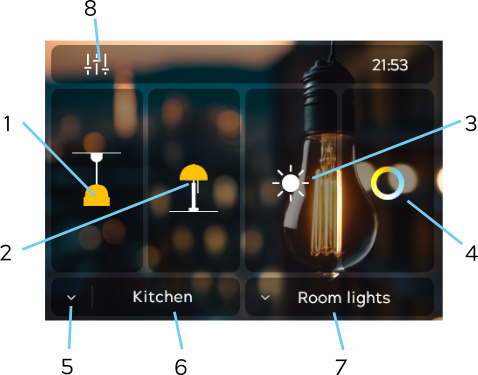
\includegraphics{main_page_numbers.png}
    \caption{Main page}%
    \end{figure}
    \bigbreak
    1. Ceiling Lights button \newline
    \textbf{Short press} - Toggle Ceiling lights ON/OFF. \newline
    \textbf{Long press} - Enter lock mode, sliders will now only effect ceiling lights. Short press to exit lock mode.
    \bigbreak
    2. Table Lights button \newline
    \textbf{Short press} - Toggle Table lights ON/OFF \newline
    \textbf{Long press} - Enter lock mode, sliders will now only effect table lights. Short press to exit lock mode.
    \bigbreak
    3. Brightness Dimmer \newline
    Control over Ceiling and Table Lights group. (More under Lights control logic below)
    \bigbreak
    4. Kelvin Dimmer \newline
    Control over Ceiling and Table Lights group. (More under Lights control logic below)
    \bigbreak
    5. Room toggle button \newline
    \textbf{Short press} - Change room.
    \bigbreak
    6. Room button \newline
    \textbf{Short press} - Enter room page for individual device control.
    \bigbreak
    7. Lights mode button \newline
    \textbf{Short press} - Toggle between Room Lights mode and All Lights mode
	  \bigbreak
    8. Scenes button. \newline
    \textbf{Short press} - Enter Scenes page. If 7 is in Room Lights mode user will enter Room Scenes. If 7 is in All Lights mode user will enter Global Scenes page.

   	\subsubsection{Lights control logic}
    The NSPanel main page might have some behavior that seems odd at first but the logic of it will be described here. The first page will affect entities in the selected room (if in room-mode) or all the configured lights (if in "All lights"-mode). The two left buttons for ceiling and table lights will always behave the same. Pressing a button that is "off" will turn on all the lights of that type. Pressing a button that is "on" will turn off all lights of that type. The sliders will always display an average value of all entities that will be affected of changes. There are few different scenarios:				

    \paragraph{One or more lights on}\mbox{} \\
    When changing the sliders, the changes will only be sent out to the lights currently on.
    If turning on a group of lights or individual lights they will be turned on to the current brightness of the slider. I.e. average dimming level in the room.
    \info{If you wish for the light to always turn on with color temperature even though you turned it off from RGB, there is a setting in the global settings.}
    
    \paragraph{No lights on}\mbox{} \\
    When changing the sliders, the changes will be sent out to all lights selected (depending on room or "all lights"-mode).
    
    \paragraph{Lock mode}\mbox{} \\
    You can lock which light to affect by pressing and holding either the ceiling or table-lights button. This will enter a special mode where changes to the sliders will only affect the selected type of lights. By pressing the same button again you can exit the "special mode". The "special mode" will also time out after a few seconds.
    
    \subsubsection{Scenes button (top left corner)}
    The settings icon in the top left corner is for entering the Scenes page. In NSPanel Manager there are both Room Scenes and Global Scenes. If you're in Room Lights mode (button in lower right corner) you will enter the Room Scenes page. If you're in All Lights mode you will enter the Global Scenes page. You'll also see that the settings icon changes when toggling between Room Lights and All Lights mode. Standard settings icon leads to Room Scenes page when pressing it. Settings icon with a roof on top leads to Global Scenes page.
    \subsubsection{Swipe down}
    You can swipe downwards when on the first page to enter the Smart Home Control page.
    This page is a work in progress. Design and funcionality is not finished or decided yet.
    \subsection{Smart Home Control page}
    Accessed by swiping down on Main page. Work in progress. Design and funcionality is not finished or decided yet.  
    \subsection{Scenes page}
    To enter Scenes page, press the settings icon in top left corner on Main page. Depending on if you're in Room Lights mode or All Lights mode you will enter Room Scenes page or Global Scenes page.
    
    Scene names that show up here are the ones you have configured in the NSPanel Manager web interface. To store a scene simply hold the save button for three seconds and the current values of the lights in the room you are in or all lights if in All Lights mode will be saved. To activate a scene and send out those saved values you just press the scene name.
    \subsection{Room page}
	Enter Room page by pressing the room name on Main page. All devices configured for that room will show up here. To control a device individually press the device name. 
    \subsection{Individual Lights page}
    All the capabilities of the chosen light will be shown on this page. If the light is RGB capable there will be an icon in the top right corner to toggle between Color Temperature mode and Color mode.´

    \clearpage
    \section{Logs}
    \label{sec:logs}
    While logs are normally sent over MQTT, any logs that are created before WiFi-connection are sent out on Serial. If you wish to see the logs going over MQTT, you can look at the topic \lstinline[language=bash]{nspanel/<panel name>/log}. If you wish to look at the logs going over serial, you can use programs like Putty. Connect to the NSPanel with the serial programmer as usual but \textbf{dont't} connect IO0 to GND. In Putty enter your serial port in the "Serial line" box and choose baud 115200. You should then be able to connect by pressing the "Open"-button. Example:
    \info{On Windows "/dev/ttyUSB0" will have to be replaced by something like "COM4". If using MacOS or Linux the port will be something similar to "/dev/ttyUSB0".}
    \begin{figure}[H]
    \centering
    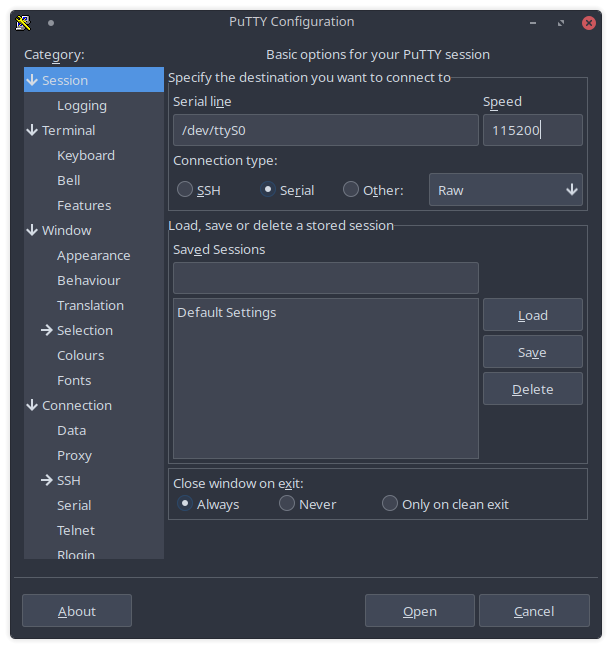
\includegraphics[scale=0.5]{putty_serial.png}
    \caption{Connecting to Serial with Putty}%
    \end{figure}

    \clearpage
    \section{Advanced setup}
    \label{sec:advanced_setup}
    \subsection{Manual Docker container setup}
    If you wish to manually build and setup the Docker container from source first clone/download this git repository. Then use the command \lstinline[language=bash]{docker build -t nspanelmanager .} while standing in the downloaded "docker"-directory. This will always be the same. To then start the container, the following command can be used:
    \begin{lstlisting}[language=bash]
    docker run --name nspanelmanager -e 'TZ=Europe/Stockholm' -v \
    "$(pwd)/data/":"/data/" \
    -d -p 8000:8000 nspanelmanager
    \end{lstlisting}
    To change the timezone, set the TZ-environment variable, for example: \lstinline[language=bash]{-e TZ=Europe/Stockholm}.
    \important{All data for NSPanel Manager is stored in the directory mapped to "/data" in the container. In this case, the "data"-directory where you are currently standing.}


    \subsection{Docker-compose container setup}
    If you wish to run NSPanel manager from docker compose you can use the below example as a template for your setup.
    \note{This example is for an x86\_64 machine placed in the Europe/Stockholm timezone. Replace image name and timezone as needed.}
    \begin{lstlisting}
    services:
      nspanelmanager:
        image: nspanelmanager/nspanelmanager-amd64
        container_name: nspanelmanager
        environment:
          - TZ=Europe/Stockholm
        volumes:
          - /nspmdata/:/data/
        ports:
          - 8000:8000
        restart: always
    \end{lstlisting}
    \important{All data for NSPanel Manager is stored in the directory mapped to "/data" in the container. In this case, the "/nspmdata/"-directory where you are currently standing.}

    \clearpage
    \section{Functional information}
    \label{sec:software_components}
    \subsection{Software components}
    There are really three software components written for the NSPanel Manager project. These are described as below:
    \begin{itemize}
      \item \textbf{Web interface:} The web interface that you interact with is built on top of the Django framework. This software gives the user an interface to interact and configure the project with. This software also manages the database with settings.
      \item \textbf{MQTT Manager:} There is a second software running in the background on the NSPanel Manager container that hosts the web interface. This component is named "MQTTManager". The MQTTManager handles all things with MQTT. It loads the config from the web interface via the API and then processes all commands from panels, state updates from Home Assistant and OpenHAB and so on. It's basically the glue that makes the panel's actions affect Home Assistant and OpenHAB. The MQTTManager is also the software that send state updates from Home Assistant and OpenHAB to the panels when changes occur.
      \item \textbf{The NSPanel firmware:} The firmware written for the NSPanel has been specifically designed to be as response and easy to use as possible. The firmware handles all communication with the TFT (Nextion) display and with MQTTManager via MQTT.
    \end{itemize}

    \subsection{Data flow}

    \begin{figure}[H]
    \centering
    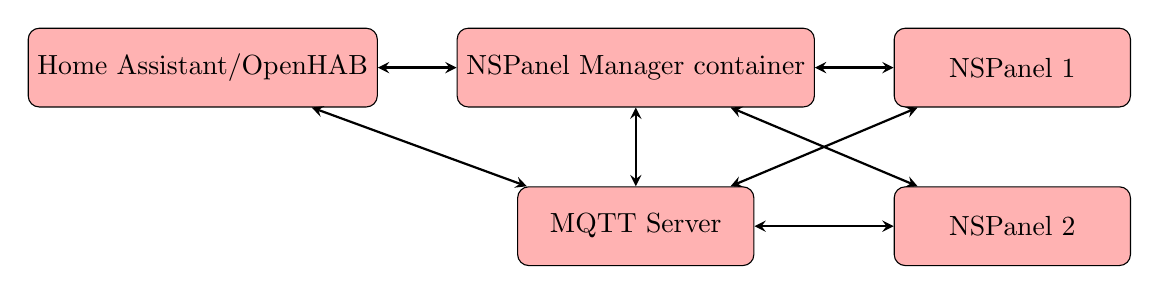
\begin{tikzpicture}
      \node (HAOpenHab) [startstop] {Home Assistant/OpenHAB};
      \node (NSPMcontainer) [startstop, right=of HAOpenHab] {NSPanel Manager container};
      \draw [doublearrow] (HAOpenHab) -- (NSPMcontainer);
      \node (MQTT) [startstop, below=of NSPMcontainer] {MQTT Server};
      \draw [doublearrow] (HAOpenHab) -- (MQTT);
      \draw [doublearrow] (NSPMcontainer) -- (MQTT);

      \node (panel1) [startstop, right=of NSPMcontainer] {NSPanel 1};
      \node (panel2) [startstop, below=of panel1] {NSPanel 2};
      \draw [doublearrow] (NSPMcontainer) -- (panel1);
      \draw [doublearrow] (NSPMcontainer) -- (panel2);
      \draw [doublearrow] (MQTT) -- (panel1);
      \draw [doublearrow] (MQTT) -- (panel2);
    \end{tikzpicture}
    \caption{NSPanel Manager data flow}%
    \end{figure}

    The data flow within NSPanel Manager might look intimidating but it's not that bad. Below is an explanation of all the arrows above.

    
    \subsubsection{Home Assistant and/or OpenHAB to/from NSPanel Manager container}
    There is two types of traffic flowing between these nodes:
    \begin{itemize}
      \item \textbf{Websocket:} A websocket connection is setup in order for the NSPanel Manager container to receive entity updates from Home Assistant and/or OpenHAB but also to sent entity commands (E.. turn light X on to 20\%). A websocket is used to speed up the communication and also to not have to poll the home automation software for information.
      \item \textbf{HTTP GET API:} The usual HTTP GET API is also used. This is used when adding entities to a room, as an example. When pressing the "Add new light" button, the NSPanel Manager container will make an HTTP GET request to gather all available entities and then send them back to the client (browser) so that the user may choose what entitiy to add to the room.
    \end{itemize}
    \subsubsection{NSPanel Manager container to/from MQTT}
    MQTT is used to send updated entity states received from the home automation software out to all NSPanels and also receive states and commands from NSPanels.
    \subsubsection{Home Assistant and/or OpenHAB to/from MQTT}
    Home Assistant and OpenHAB can leverage the MQTT integration through "Home Assistant MQTT Auto-discovery" (which OpenHAB can also use) to auto-discover NSPanels and automatically register entities for panel temperature reading, panel relays, screen state and so on.
    \subsubsection{NSPanel Manager container to/from NSPanels}
    The configuration of lights, scenes and so on does not reside on each panel. The panel only has localy the bare minimum configuration for setup. When the panel starts and has connected to WiFi it will do a HTTP GET request to the NSPanel Manager container in order to receive all configuration of entities, screen brightness and really, all settings available in the NSPanel Manager web interface.
    \subsubsection{MQTT to/from NSPanels}
    Each NSPanel send states (E.g. temperature) and commands (E.g. turning on a light) over MQTT for the NSPanel Manager container to pickup. The panel also received commands, E.g. turn on relay 1, turn on screen and so on.

    \subsection{MQTT Topics}
    Below table is a description of all MQTT topics that might be of use by a user. Replace <panel\_name> with the friendly name of your NSPanel:
    \begin{table}[H]
    \begin{tabular}{|l|l|l|}
    \hline
    \textbf{Topic} & \textbf{Payload}  & \textbf{Description}  \\ \hline
    nspanel/<panel\_name>/screen\_cmd & 1 or 0 & Send a 1 or 0 to turn on/off the display. \\ \hline
    nspanel/<panel\_name>/screen\_state & 1 or 0 & Current state of the screen. \\ \hline
    nspanel/<panel\_name>/brightness & 1 to  100 & Control the brightness of the screen. \\ \hline
    nspanel/<panel\_name>/brightness\_screensaver & 0 to  100 & Control the brightness of the screensaver. \\ \hline
    nspanel/<panel\_name>/r1\_cmd & 1 or 0 & Send a 1 or 0 to turn on/off relay 1. \\ \hline
    nspanel/<panel\_name>/r1\_state & 1 or 0 & The current state of relay 1. \\ \hline
    nspanel/<panel\_name>/r2\_cmd & 1 or 0 & Send a 1 or 0 to turn on/off relay 2. \\ \hline
    nspanel/<panel\_name>/r2\_state & 1 or 0 & The current state of relay 2. \\ \hline
    nspanel/<panel\_name>/temperature\_state & Current temperature & The current temperature reading. \\ \hline
    nspanel/<panel\_name>/screensaver\_mode & screensaver mode & \parbox[t]{0.25\textwidth}{Select what screensaver to display Choose from the following:\\ with\_background,\\ without\_background,\\ datetime\_with\_background,\\ datetime\_without\_background\\ or no\_screensaver} \\ \hline
    nspanel/<panel\_name>/log & Log message & The panel will send live logs on this topic. \\ \hline
    \end{tabular}
    \end{table}

    There are more topics that are used internally, these are:

    \begin{table}[H]
    \centering
    \resizebox{\textwidth}{!}{\begin{tabular}{|l|l|L{8cm}|}
    \hline
    \textbf{Topic} & \textbf{Payload}  & \textbf{Description}  \\ \hline
    nspanel/entities/<type>/<id>/state\_<attribute> & The value of the attribute & An update of entity state value sent out by MQTTManager. Example: nspanel/entities/light/42/state\_kelvin \\ \hline
    nspanel/status/time & Time as a string & Current time sent by MQTTManager. \\ \hline
    nspanel/status/weather & JSON & A JSON representation of the current weather and weather forecast. \\ \hline
    nspanel/<panel\_name>/status\_report & JSON & JSON payload with current state of the panel. \\ \hline
    nspanel/<panel\_name>/status & JSON & JSON payload with current online/offline state of the panel. \\ \hline
    nspanel/<panel\_name>/command & JSON & JSON payload with a command for the panel to execute. \\ \hline
    nspanel/mqttmanager/command & JSON & JSON payload from panel with a command for MQTTManager to perform. \\ \hline
    \end{tabular}}
    \end{table}


\end{document} % This is the end of the document
